Consider the following system.
\begin{center}
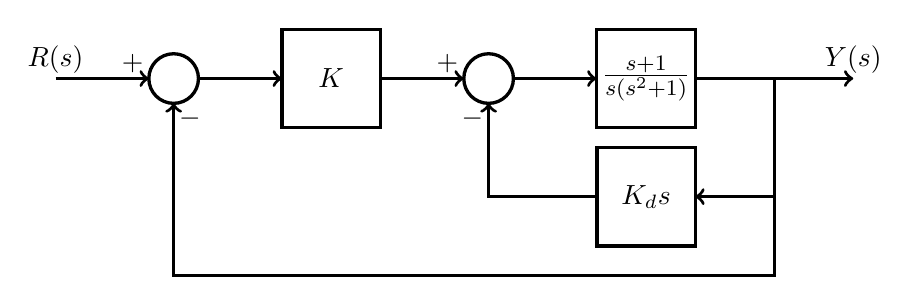
\begin{tikzpicture}[scale=1,inner sep=0pt,outer sep=0pt,very thick,
sysblock/.style={draw,rectangle,inner sep=2pt,minimum width=1.25cm,minimum height=1.25cm,very thick}]
\draw (1.5,0) node[draw,circle] (sum1) {$\rule{0pt}{18pt}$};
\draw (3.5,0) node[sysblock] (Kp) { $\large K$};
\draw (5.5,0) node[draw,circle] (sum2) {$\rule{0pt}{18pt}$};
\draw (7.5,0) node[sysblock] (G) {\large $\frac{s+1}{s(s^2+1)}$};
\draw (7.5,-1.5) node[sysblock] (Kd) {$K_{d}s$};
\draw[->] (0,0) node[above=2pt] {$R(s)$} -- (sum1.180) node[above left=2pt] {$+$};
\draw[->] (sum1.0) --  (Kp);
\draw[->] (Kp) -- (sum2.180) node[above left=2pt] {$+$};
\draw[->] (sum2.0) -- (G.180);
\draw[->] (G.0) -- ++(2,0) node[above=2pt] {$Y(s)$};
\draw[->] (G.0) ++(1,0) |- (Kd.0);
\draw[->] (Kd.180) -| (sum2.-90) node[below left=2pt] {$-$};
\draw[->] (G.0) ++(1,0) -- ++(0,-2.5) -| (sum1.-90) node[below right=2pt] {$-$};
\end{tikzpicture}
\end{center}
\begin{enumerate}[(a)]
\item Sketch the root locus (of closed loop poles as $K$ varies) if $K_{d}=0$
\item Sketch the root locus (of closed loop poles as $K$ varies) if $K_{d}=2$
\item In which cases, if any, does there exist a $K$ such that the closed loop system is stable?
\end{enumerate}
